\chapter{Código fonte da nuvem de palavras sobre live coding}\label{app:C}

Apresentamos no exemplo A.1 o código-fonte, em linguagem python, utilizado para extração parcial do espaço conceitual da pesquisa (\autoref{fig:nuvemlivecoding}, p.~\pageref{fig:nuvemlivecoding}). A biblioteca utilizada, \emph{Wordcloud}, pode ser encontrada em \url{https://github.com/amueller/word_cloud}.

O Código abaixo considera a seguinte situação: é possível converter um arquivo de texto em formato \emph{.pdf} para formato \emph{.txt}. Feita a conversão, é possível realizar um levantamento estatístico das palavras mais usadas (o que pode, parcialmente, indicar idéias e conceitos).

 Existem programas online, como o encontrado no link \url{http://convertonlinefree.com/PDFToTXTEN.aspx}, que realizam a conversão. É necessária a correção de alguns erros de caracteres (ver \autoref{fig:utf8}). Além disso, informações de cabeçalho, códigos-fontes, e outros elementos de editoração, foram descartados por considerarmos que não eram parte do corpo textual. Em outras palavras, descartamos palavras que não faziam parte de um discurso de texto, ou atrapalhavam o processo de criação da imagem. O que por sí não resolve todos os problemas, mas auxilia na elaboração da imagem.

\begin{figure}[!h]
  \centering
  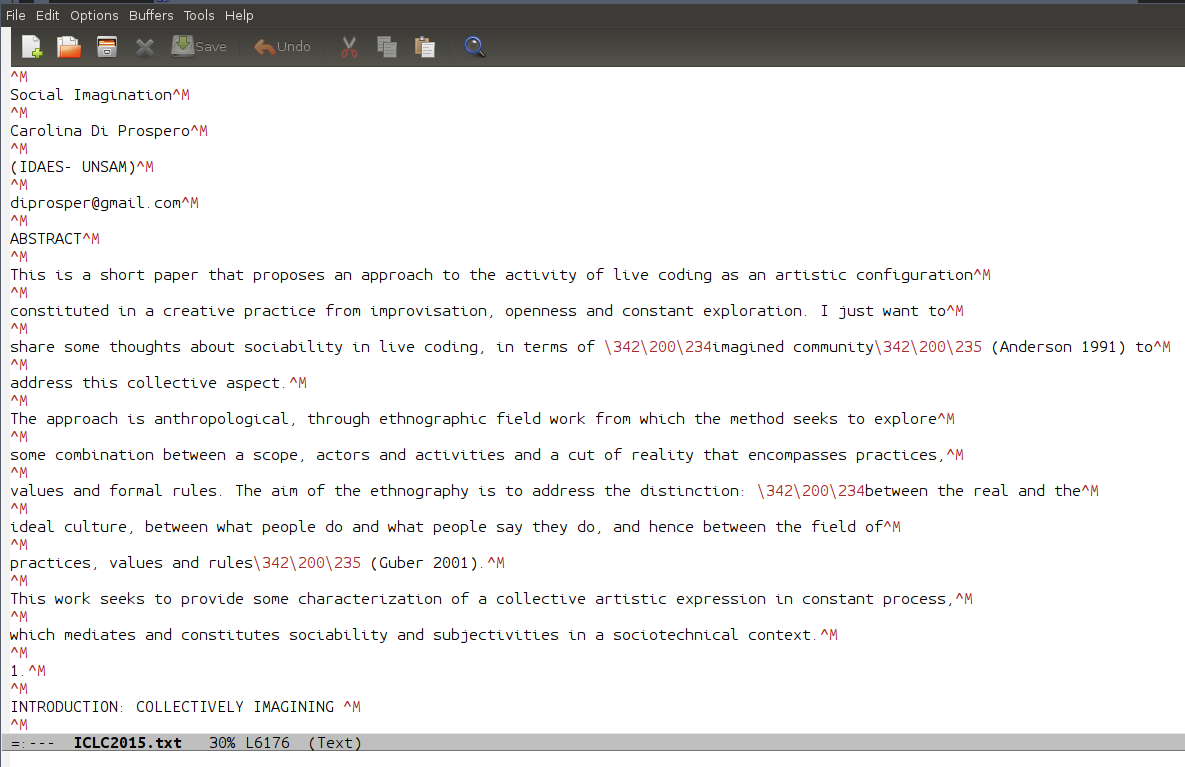
\includegraphics[scale=0.3]{imagens/utf8.png}
  \caption{Resultado da conversão do arquivo \emph{pdf} para \emph{txt} resulta em problemas de codificação que necessitaram ser corrigidos por comparação com o arquivo original. \textbf{Fonte}: autor.}
  \label{fig:utf8}
\end{figure}


\begin{example}{Código-fonte que utiliza a biblioteca wordcloud}  
\begin{minted}{python}
# Bibliotecas utilizadas
from urllib2 import urlopen
from bs4 import *
import re
import datetime
from iso import *
import matplotlib.pyplot as plt

from wordcloud import WordCloud
    
# Abra o arquivo em modo de leitura
t = open("ICLC2015.txt", "r").read()

# Gere uma nuvem de palavras
wc = WordCloud().generate(t)
    
# Mostre a imagem gerada com o matplotlib
# levando em conta as frequencias das palavras
plt.figure()
plt.imshow(wc)
plt.axis("off")
plt.show()
\end{minted}
\label{cod:nuvem}
\end{example}